\chapter{Appendix}
\begin{figure}[h!]
	\centering
	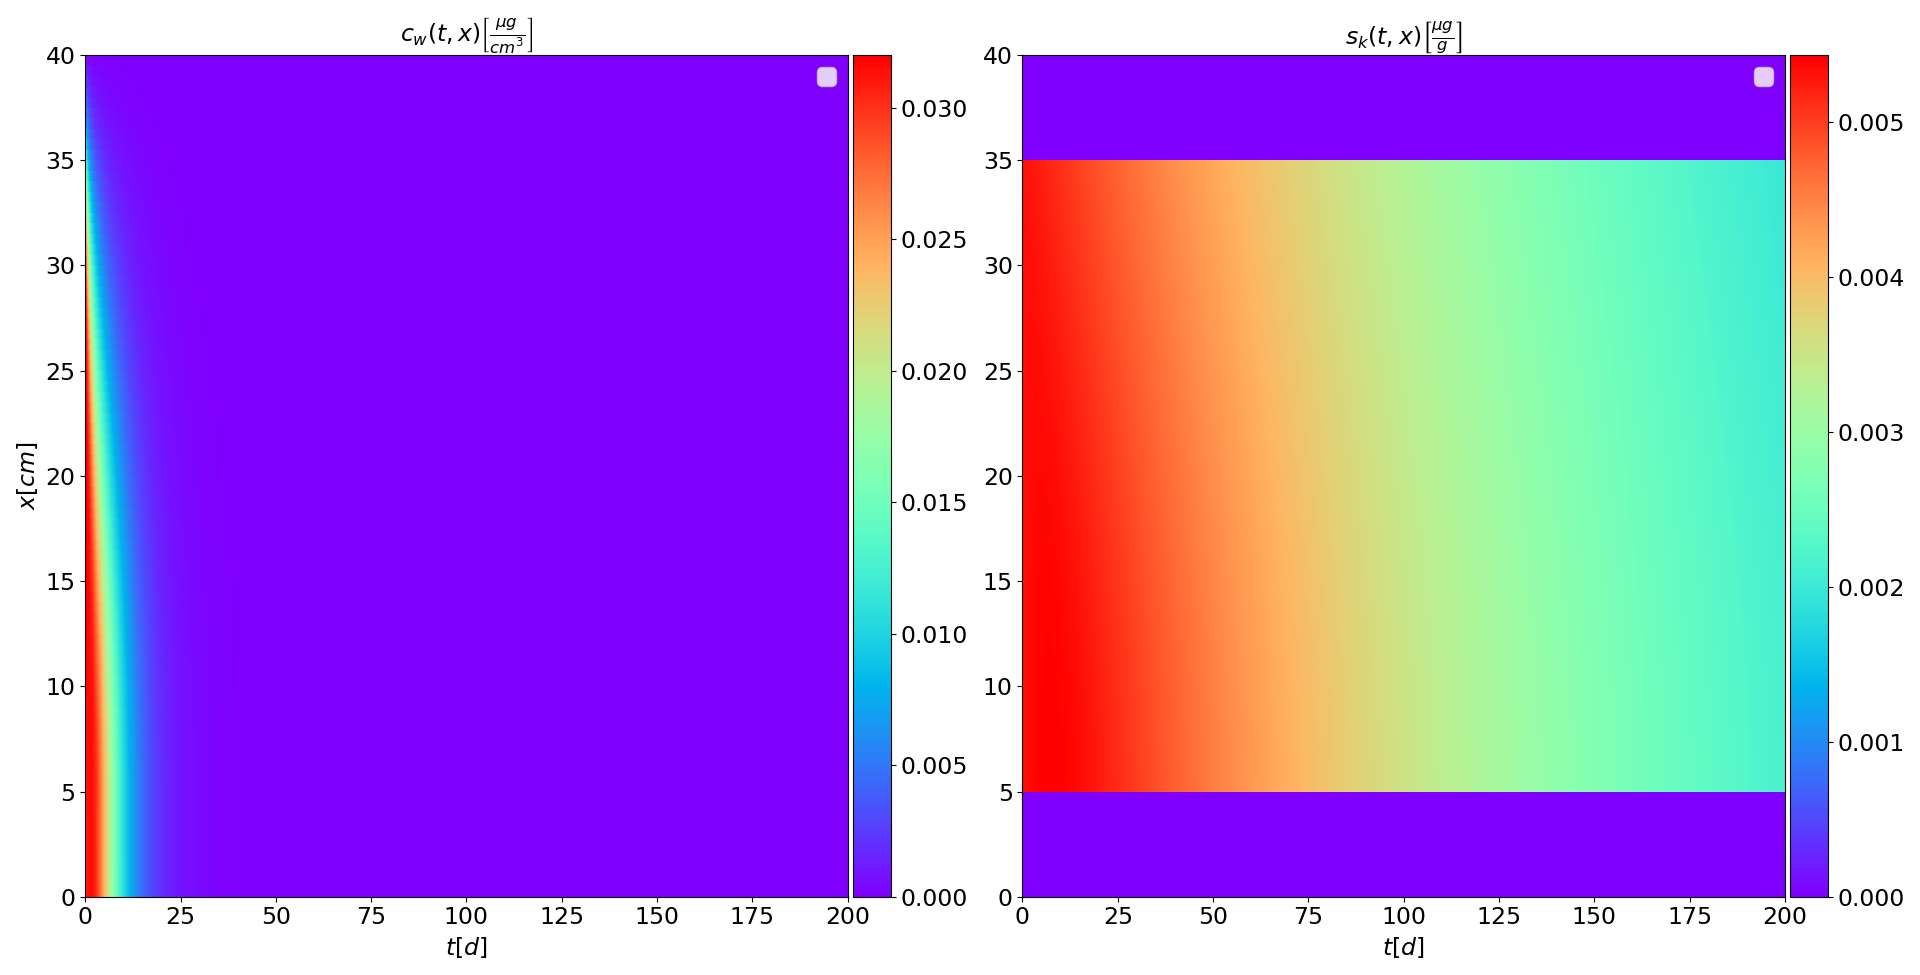
\includegraphics[scale=0.3]{images/sol_fd_sand.png}
\caption[Further FD solution]{FD solution of the dissolved concentration (left) and kinetically sorbed concentration (right). Used parameters are $n_e = 0.4$, $\rho = 1.58 \frac{g}{cm^3}$, $k_d = 4.5 \frac{cm^3}{g}$, $\beta = 0.98$, $f = 0.93$, $\alpha_k = 0.005 \frac{1}{d}$, $D_e = 2.5\frac{cm^2}{d}$, $\alpha_l = 9cm$, $v=50\frac{cm}{d}$, $c_{init} = 0.032 \frac{\mu g}{cm^3}$, $s_{k, init} = 0.0053 \frac{\mu g}{g}$, $T_{MAX} = 200d$, $T_{STEPS} = 1000000$, $X_{LENGTH} = 40cm$, $X_{STEPS} = 80$, $top = 10$, $bot=70$, $n_{e, sand} = 0.31$, $\alpha_{l, sand} = 5cm$, $v_{sand} = 64.516 \frac{cm}{d}$, $D$ was calculated as described in eq. \ref{eq:d_etodisp}.}
\label{fig:hyd_app_1}
\end{figure}
\begin{figure}
	\centering
	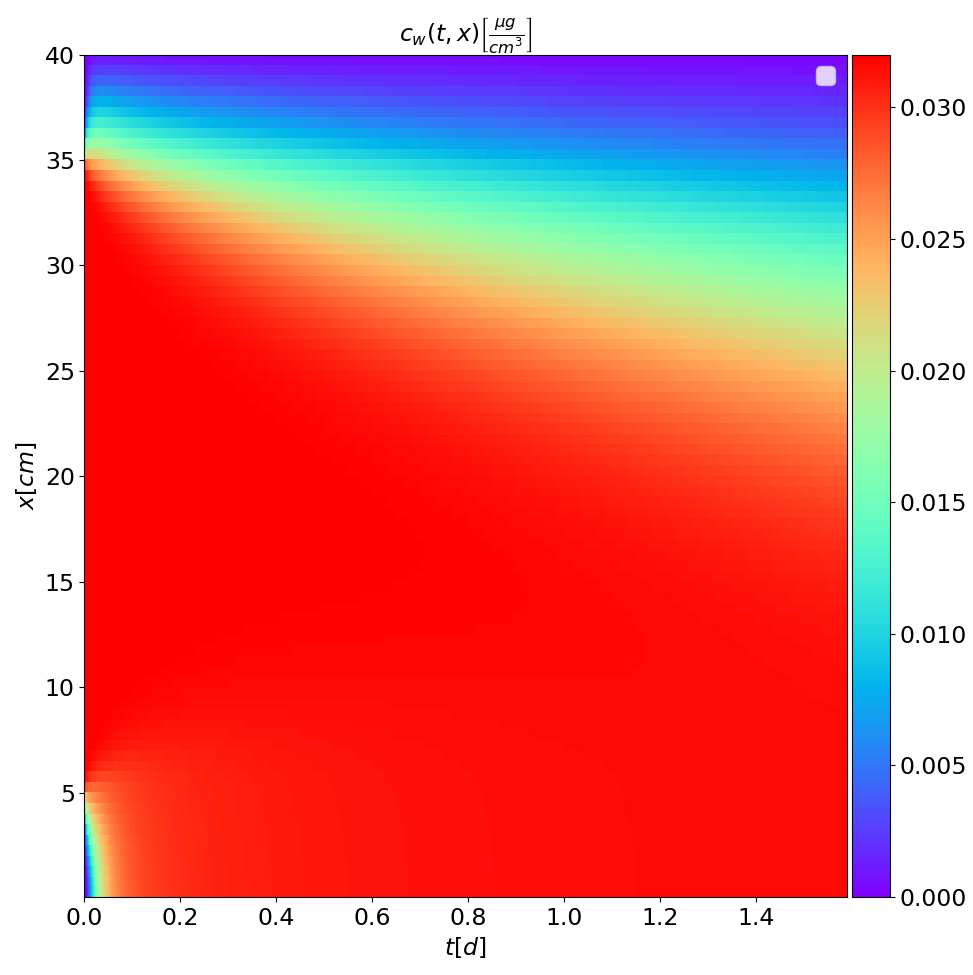
\includegraphics[scale=0.3]{images/sol_fd_sand_1d.png}
\caption[The first days of a FD solution]{The first days of a FD solution. Parameters were the same as in Fig. \ref{fig:hyd_app_1}.}
\label{fig:hyd_app_2}
\end{figure}
\FloatBarrier
\begin{figure}
	\centering
	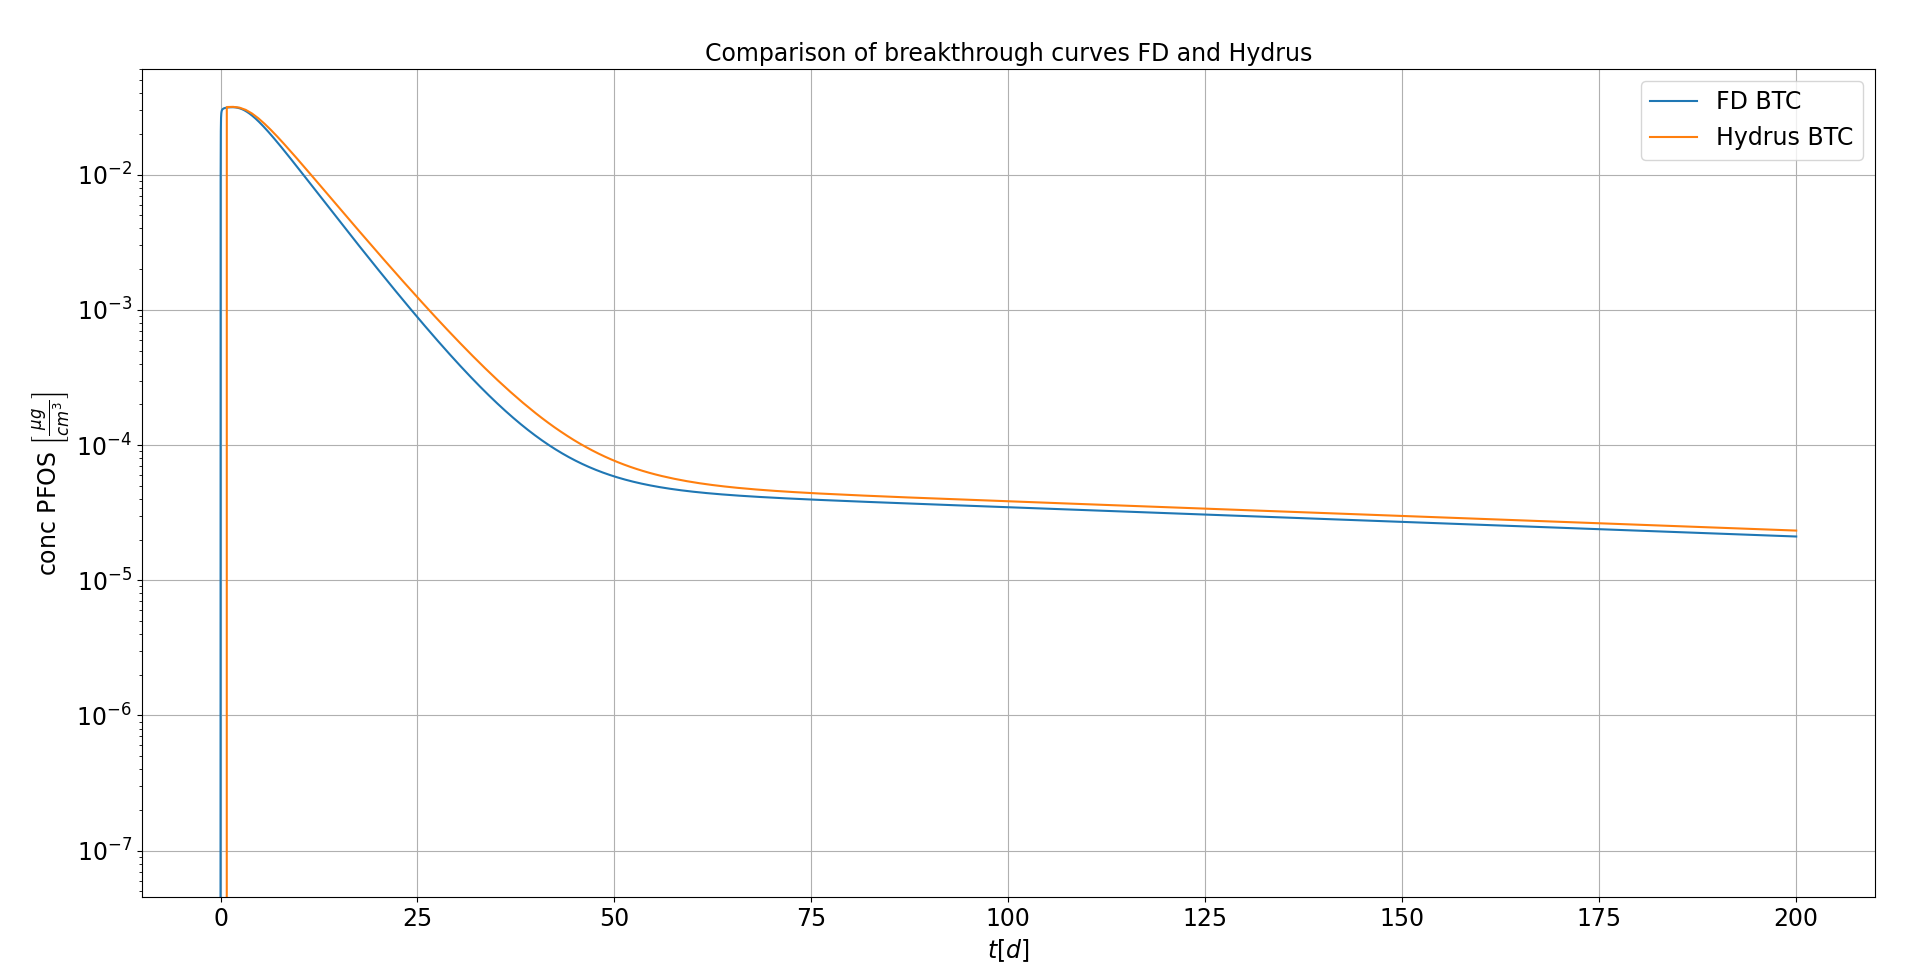
\includegraphics[scale=0.3]{images/hyd_fd_btc_c_sand.png}
\caption[Additional comparison of Hydrus and FD BTCs]{Comparison of BTCs, calculated by FD and Hydrus, sand layers included. Parameters were the same as in Fig. \ref{fig:hyd_app_1}.}
\label{fig:hyd_app_4}
\end{figure}
\begin{figure}
	\centering
	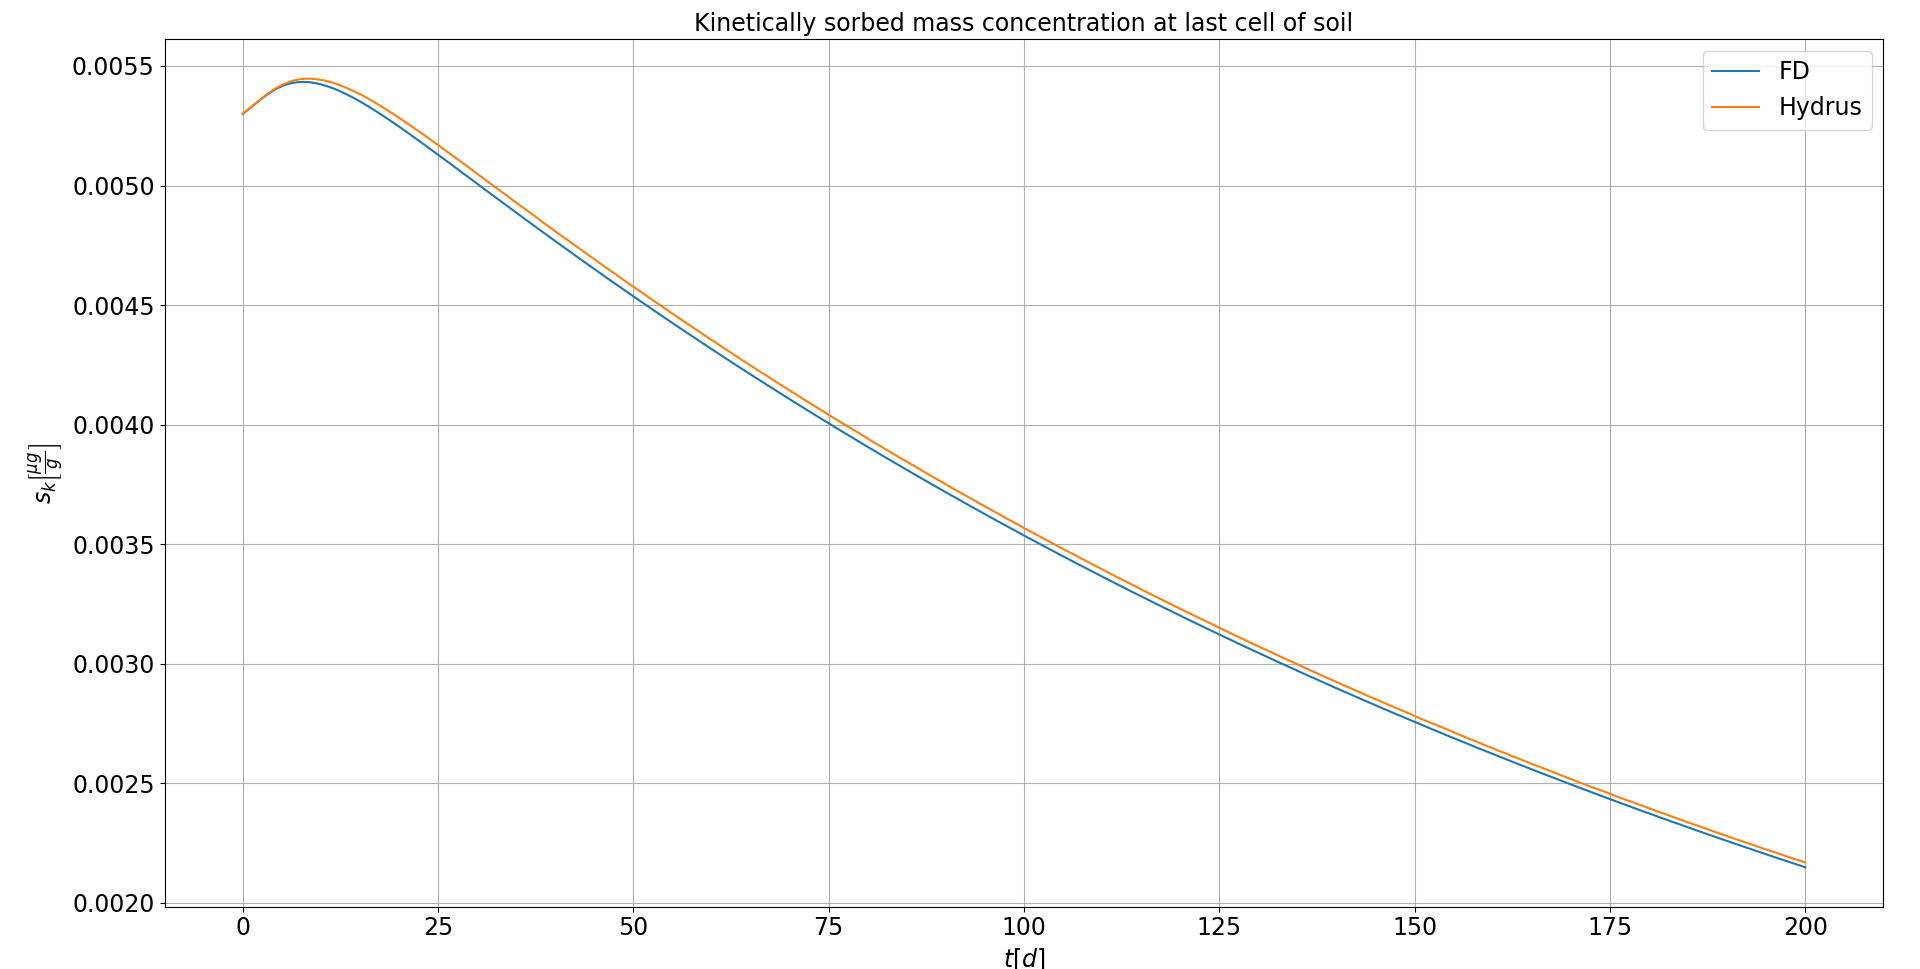
\includegraphics[scale=0.26]{images/hyd_fd_btc_sk_sand.png}
\caption[Additional comparison of Hydrus and FD kinetically sorbed concentrations]{Comparison of kinetically sorbed concentration, calculated by FD and Hydrus, sand layers included. The bottom row of the contaminated soil is considered. Parameters were the same as in Fig. \ref{fig:hyd_app_1}.}
\label{fig:hyd_app_5}
\end{figure}
\begin{figure}
	\centering
	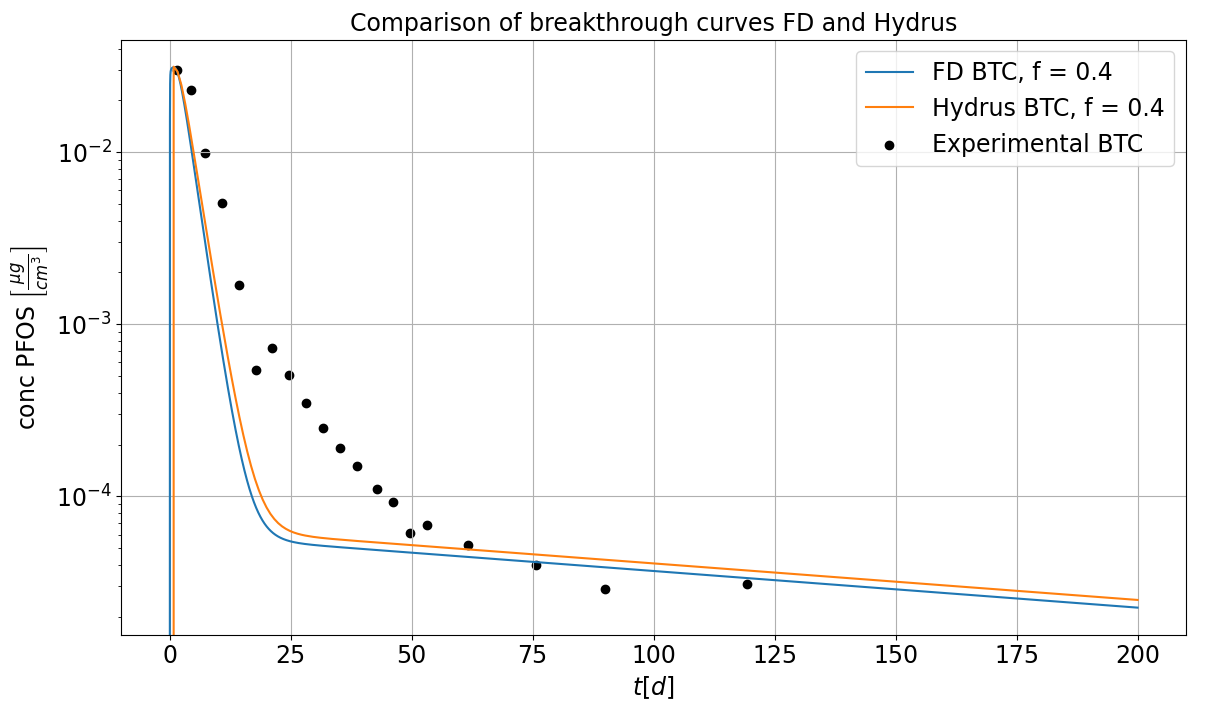
\includegraphics[scale=0.43]{images/hyd_pde_exp_0.4.png}
\caption[Comparison of experimental, Hydrus and FD BTCs, $f=0.4$]{Comparison of experimental, Hydrus and FD BTC. Parameters: $n_e = 0.4$, $\rho = 1.58 \frac{g}{cm^3}$, $k_d = 4.5 \frac{cm^3}{g}$, $\beta = 0.98$, $f = 0.4$, $\alpha_k = 0.005 \frac{1}{d}$, $D_e = 2.55\frac{cm^2}{d}$, $\alpha_l = 9cm$, $v=78.9\frac{cm}{d}$, $c_{init} = 0.032\frac{\mu g}{cm^3}$, $s_{k, init} = 0.005337 \frac{\mu g}{g}$, $T_{MAX} = 200d$, $T_{STEPS} = 230000$, $X_{LENGTH} = 55cm$, $X_{STEPS} = 56$, $top = 7$, $bot = 49$, $n_{e,sand} = 0.31$, $\alpha_{l,sand} = 5cm$, $v_{sand} = 101.80645 \frac{cm}{d}$, Hydrus settings like Bierbaum et al. ($f = 0.4$).}
\label{fig:hyd_pde_exp_0.4}
\end{figure}
\begin{figure}
	\centering
	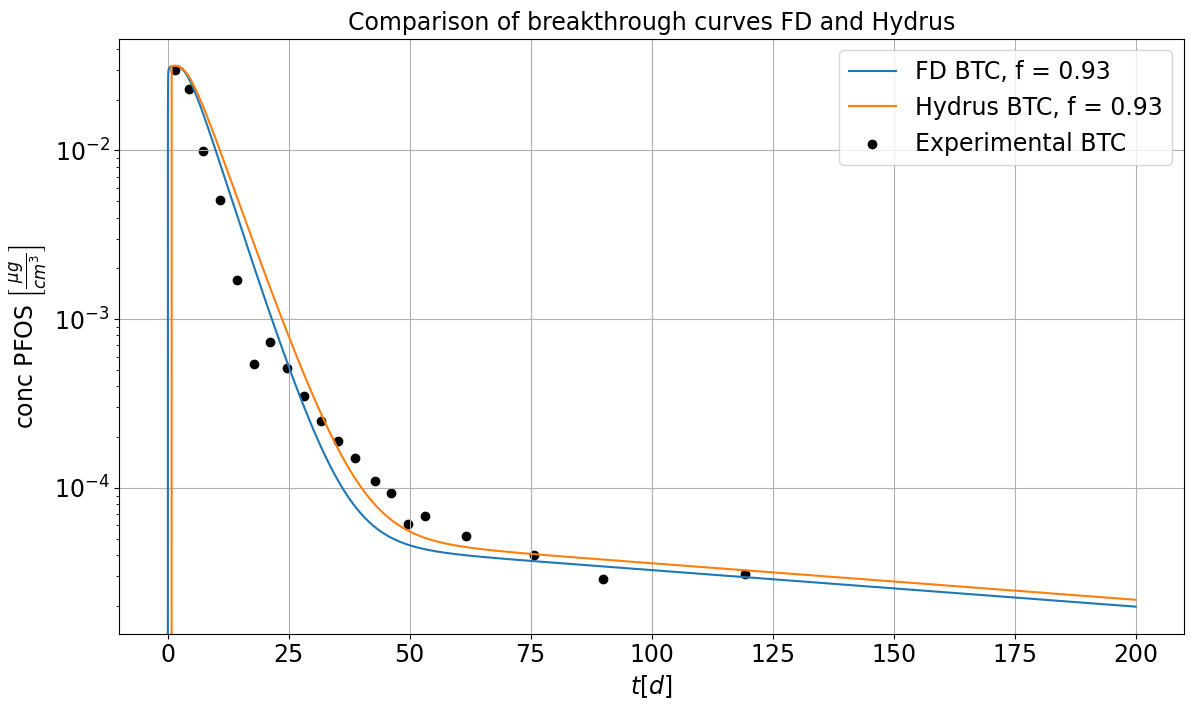
\includegraphics[scale=0.5]{images/hyd_pde_exp_0.93.png}
\caption[Comparison of experimental, Hydrus and FD BTCs, $f=0.93$]{Comparison of experimental, Hydrus and FD BTCs with $f=0.93$. Parameters were the same as in Fig. \ref{fig:hyd_pde_exp_0.4}.}
\label{fig:hyd_pde_exp_0.93}
\end{figure}
\begin{figure}
	\centering
	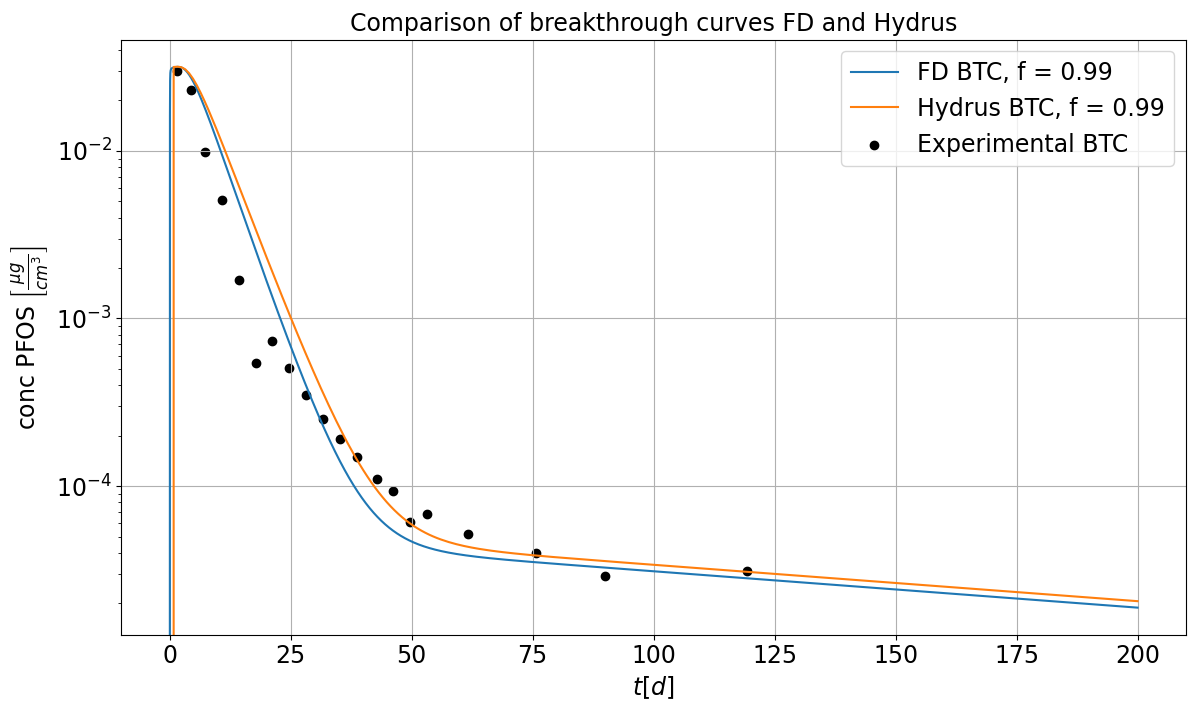
\includegraphics[scale=0.5]{images/hyd_pde_exp_0.99.png}
\caption[Comparison of experimental, Hydrus and FD BTCs, $f= 0.99$]{Comparison of experimental, Hydrus and FD BTCs with $f=0.99$. Parameters were the same as in Fig. \ref{fig:hyd_pde_exp_0.4}.}
\label{fig:hyd_pde_exp_0.99}
\end{figure}

\begin{figure}
    \centering
    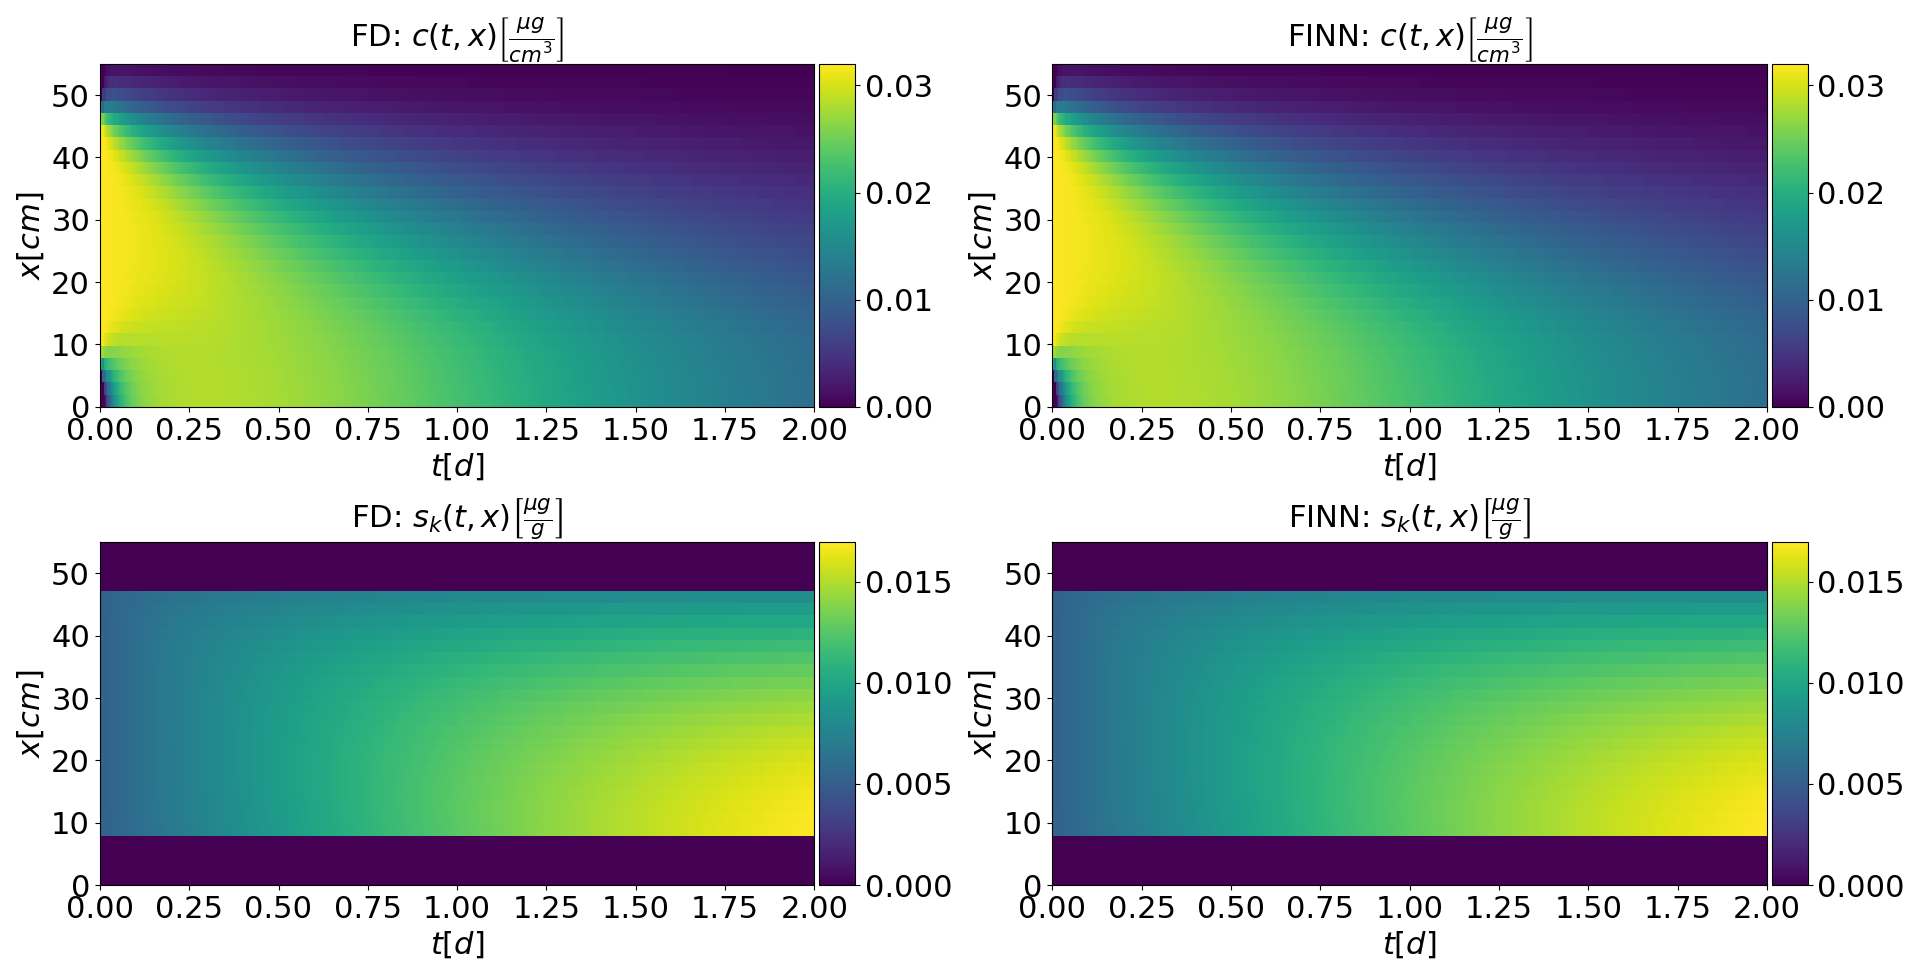
\includegraphics[scale=0.3]{images/res_ov_synt_pf.png}
    \caption[Comparison of FD and FINN solution, run b]{Comparison of FD and FINN predicted $c$ and $s_k$, run b.}
    \label{fig:res_ov_synt_pf}
\end{figure}
\begin{figure}
    \centering
    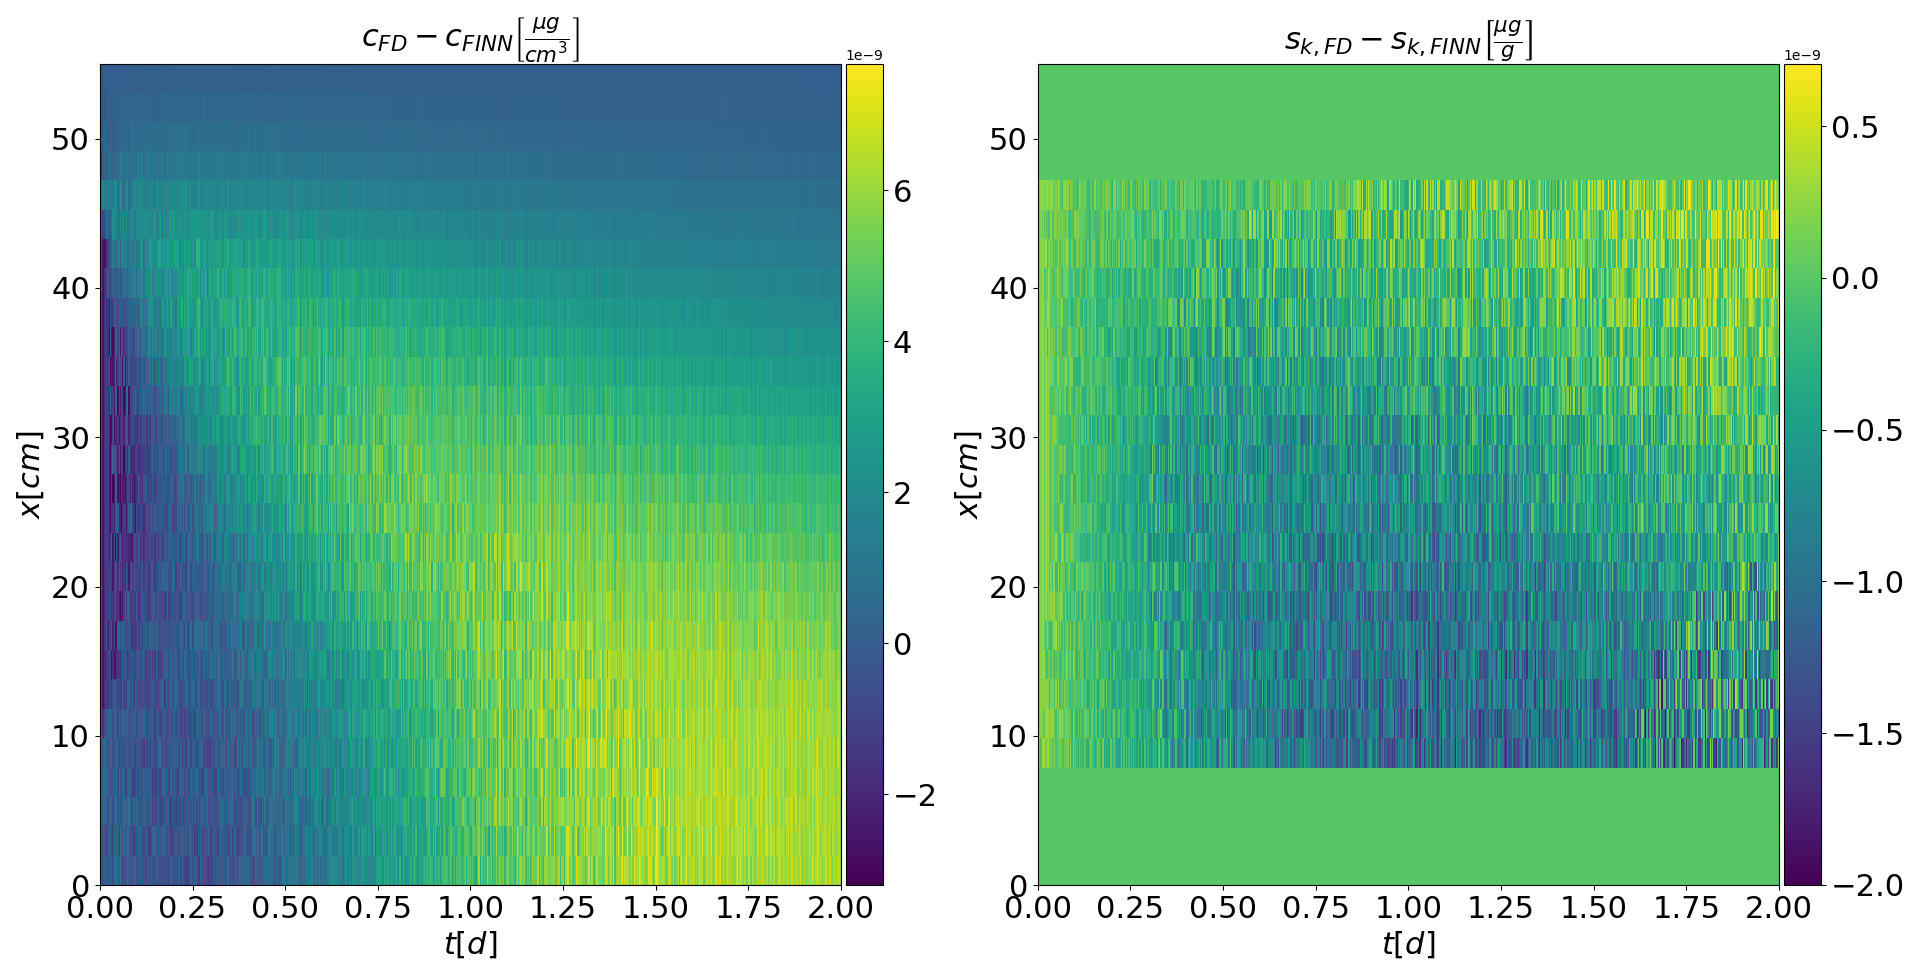
\includegraphics[scale=0.3]{images/res_diff_synt_pf.png}
    \caption[Difference FD and FINN solution, run b]{Difference of FD and FINN predicted $c$ and $s_k$, run b.}
    \label{fig:res_diff_synt_pf}
\end{figure}
\begin{figure}
    \centering
    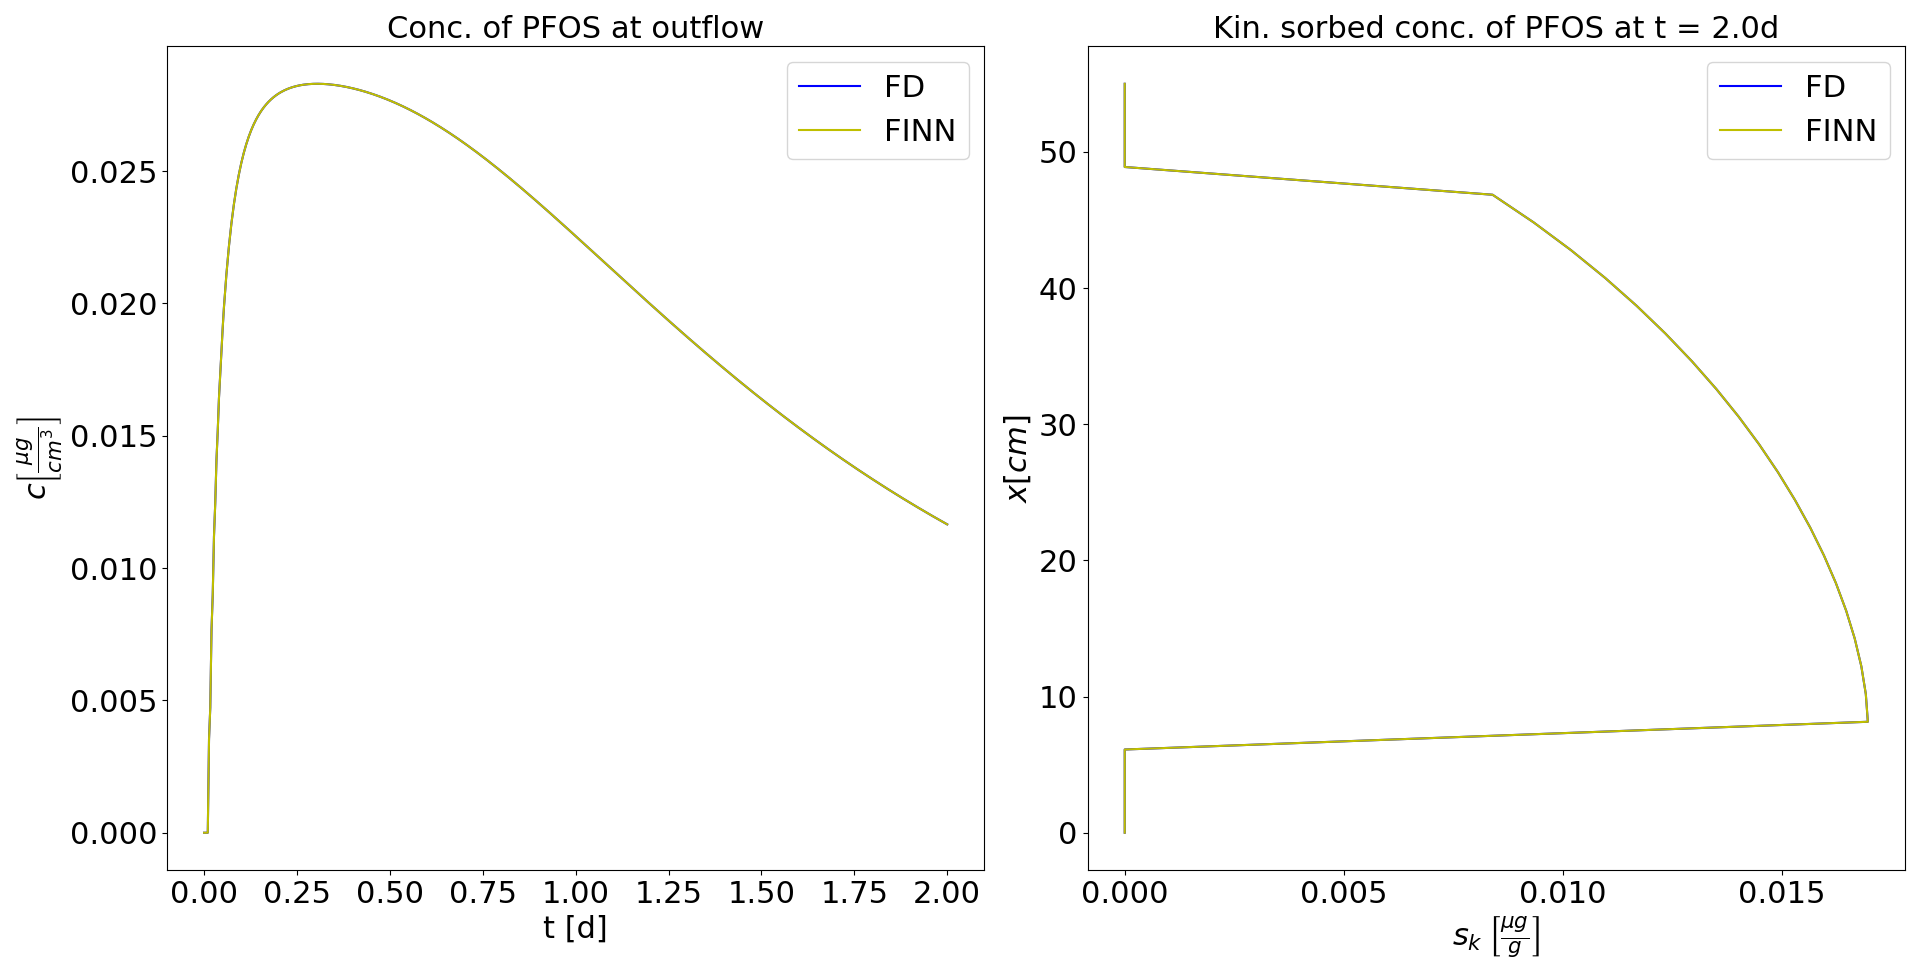
\includegraphics[scale=0.3]{images/res_btc_synt_pf.png}
    \caption[Comparison of FD and FINN BTCs, run b]{BTC of PFOS given by FD and approximated by FINN (left), Right: Kin. sorbed concentration of PFOS at $t_{end}$ (right), run b.}
    \label{fig:res_btc_synt_pf}
\end{figure}
\begin{figure}
    \centering
    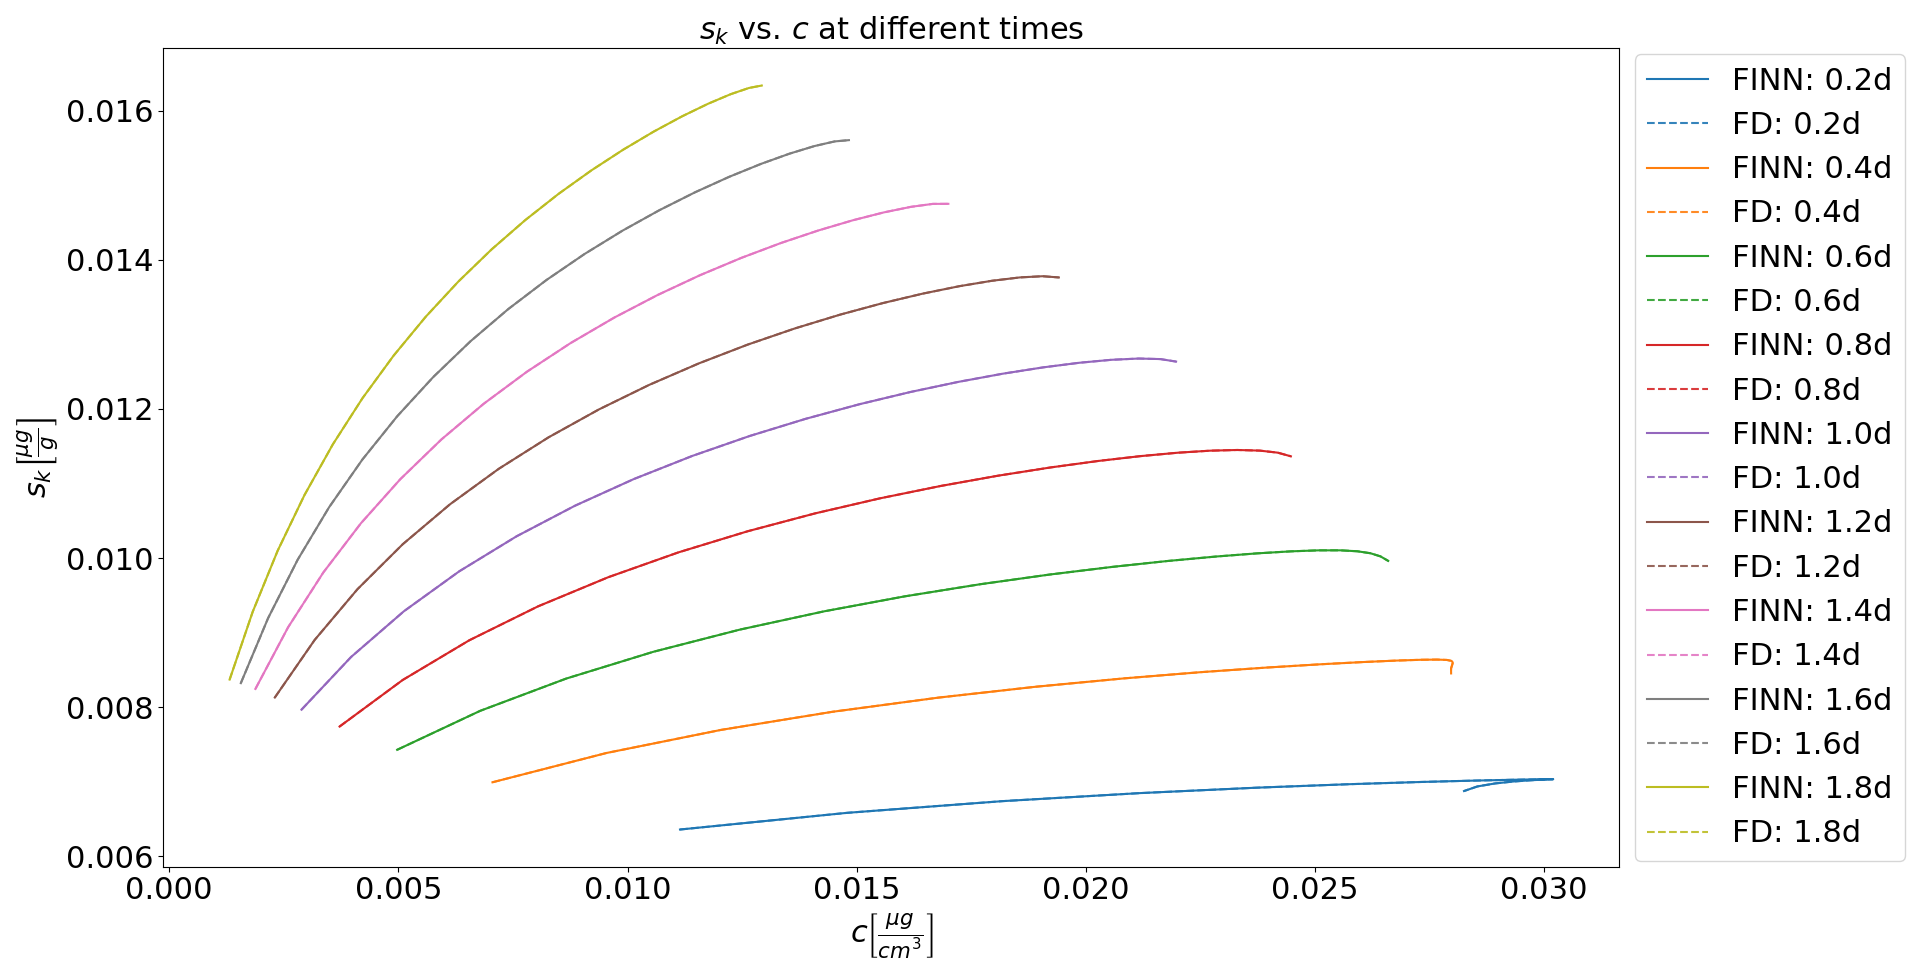
\includegraphics[scale=0.3]{images/res_sorp_synt_pf.png}
    \caption[Comparison of FD and FINN sorption behavior, run b]{The unknowns $s_k$ and $c$ of the FINN solution at fixed time steps, run b.}
    \label{fig:res_sorp_synt_pf}
\end{figure}
\begin{figure}
	\centering
	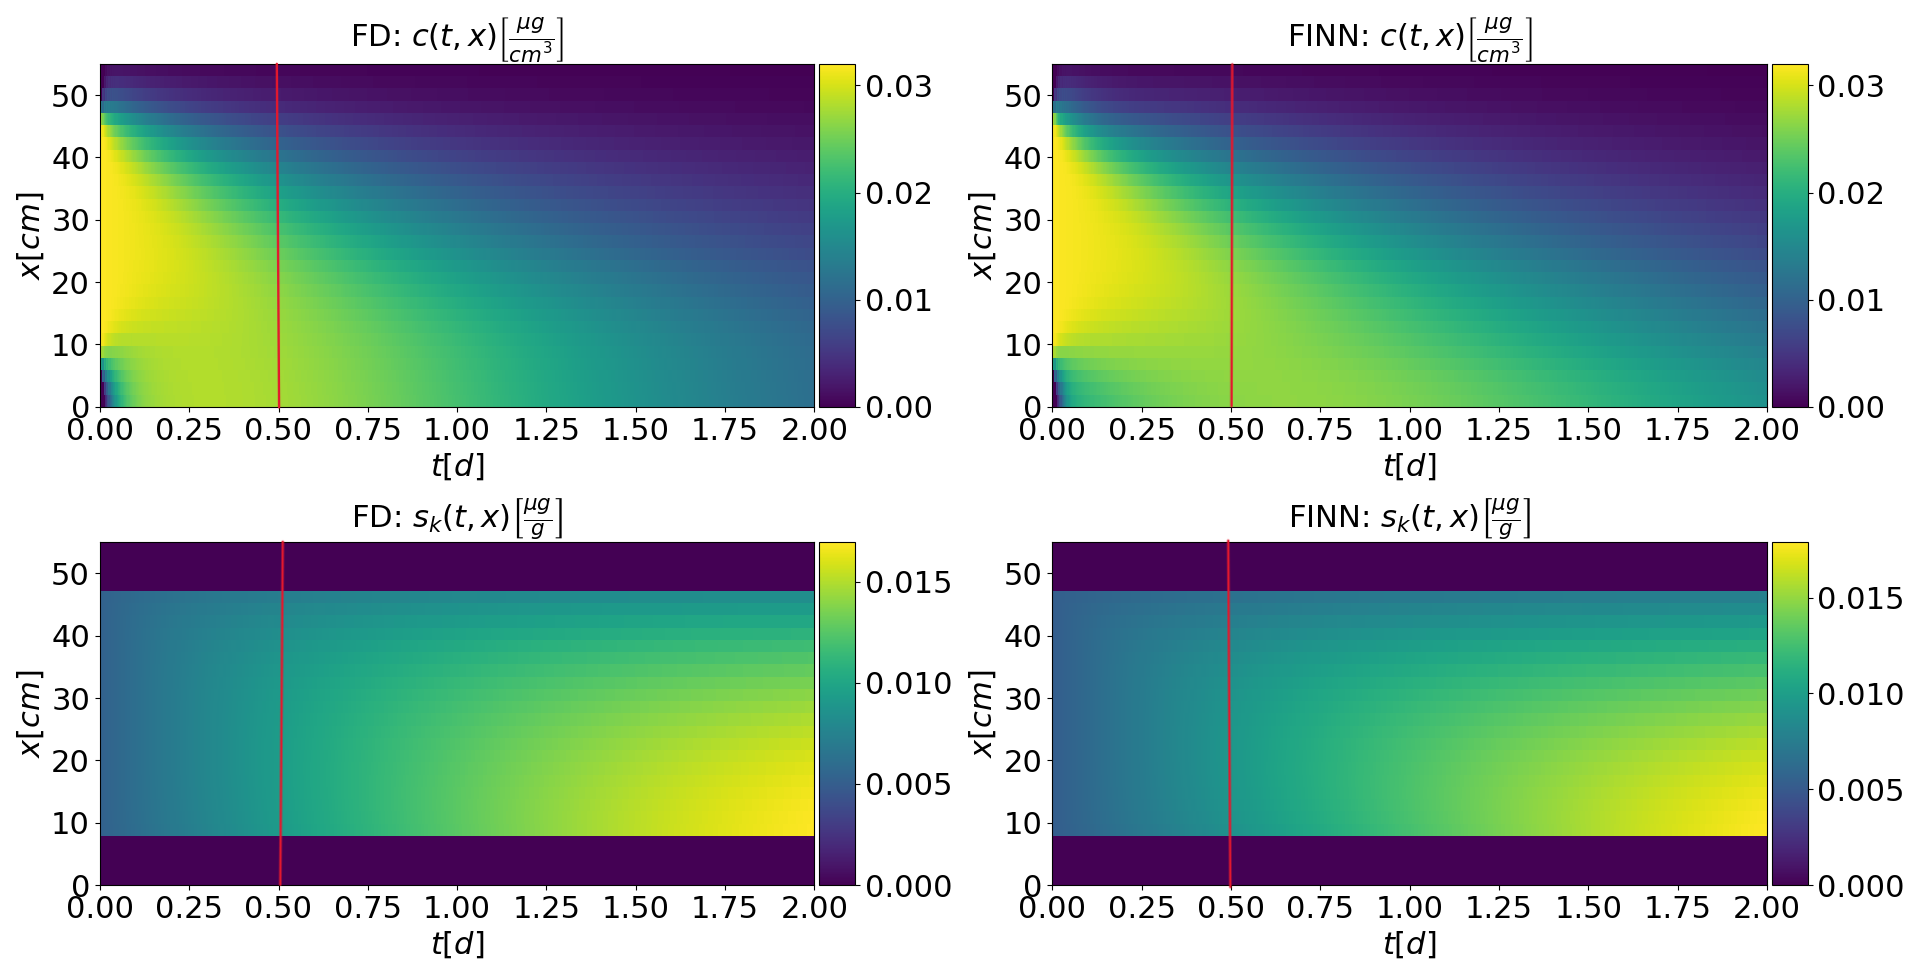
\includegraphics[scale=0.3]{images/res_ov_synt_FGR_300_m.png}
\caption[Additional comparison of FINN and FD solution]{Additional comparison of $c$ and $s_k$ calculated by FD and FINN, red line marks end of the training data set, 300 training epochs. Other settings as in run e.}
\label{fig:res_ov_synt_FGR_300_m}
\end{figure}
\begin{figure}
	\centering
	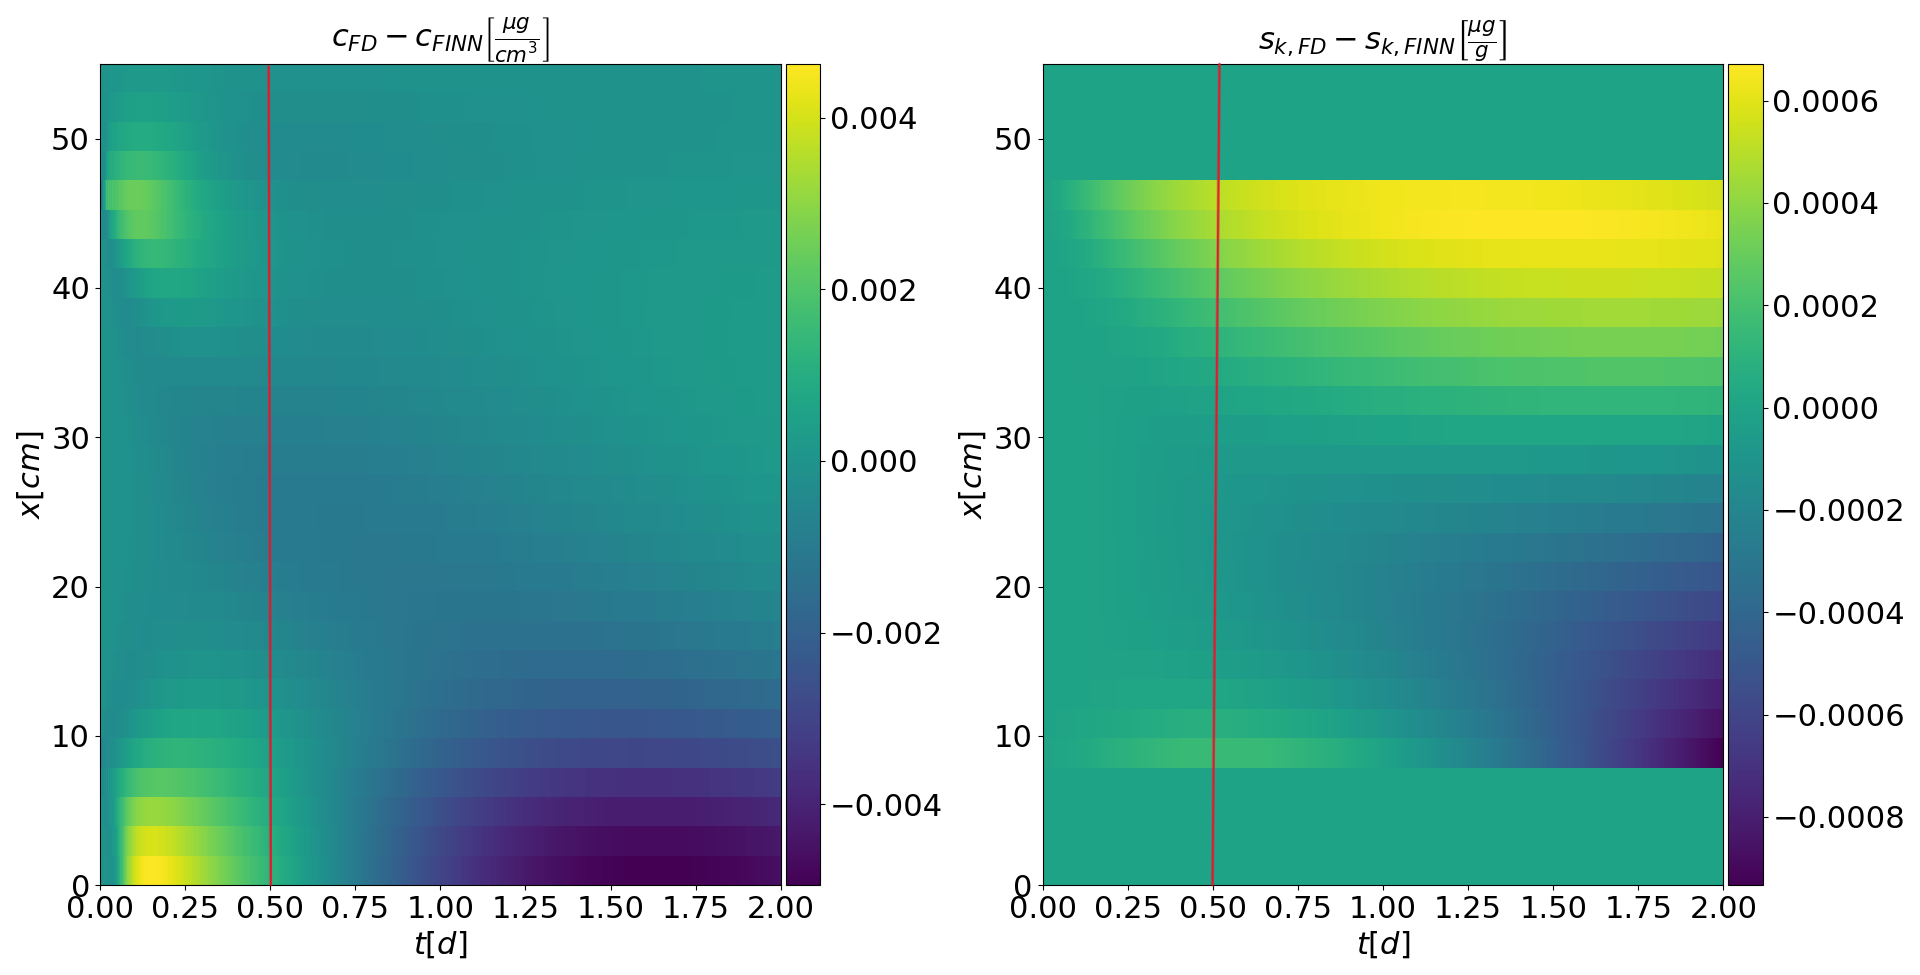
\includegraphics[scale=0.3]{images/res_diff_synt_FGR_300_m.png}
\caption[Additional difference of FINN and FD]{Difference FD and FINN predicted $c$ and $s_k$, red line marks end of the training data set, 300 training epochs. Other settings as in run e.}
\label{fig:res_diff_synt_FGR_300_m}
\end{figure}
\begin{figure}
	\centering
	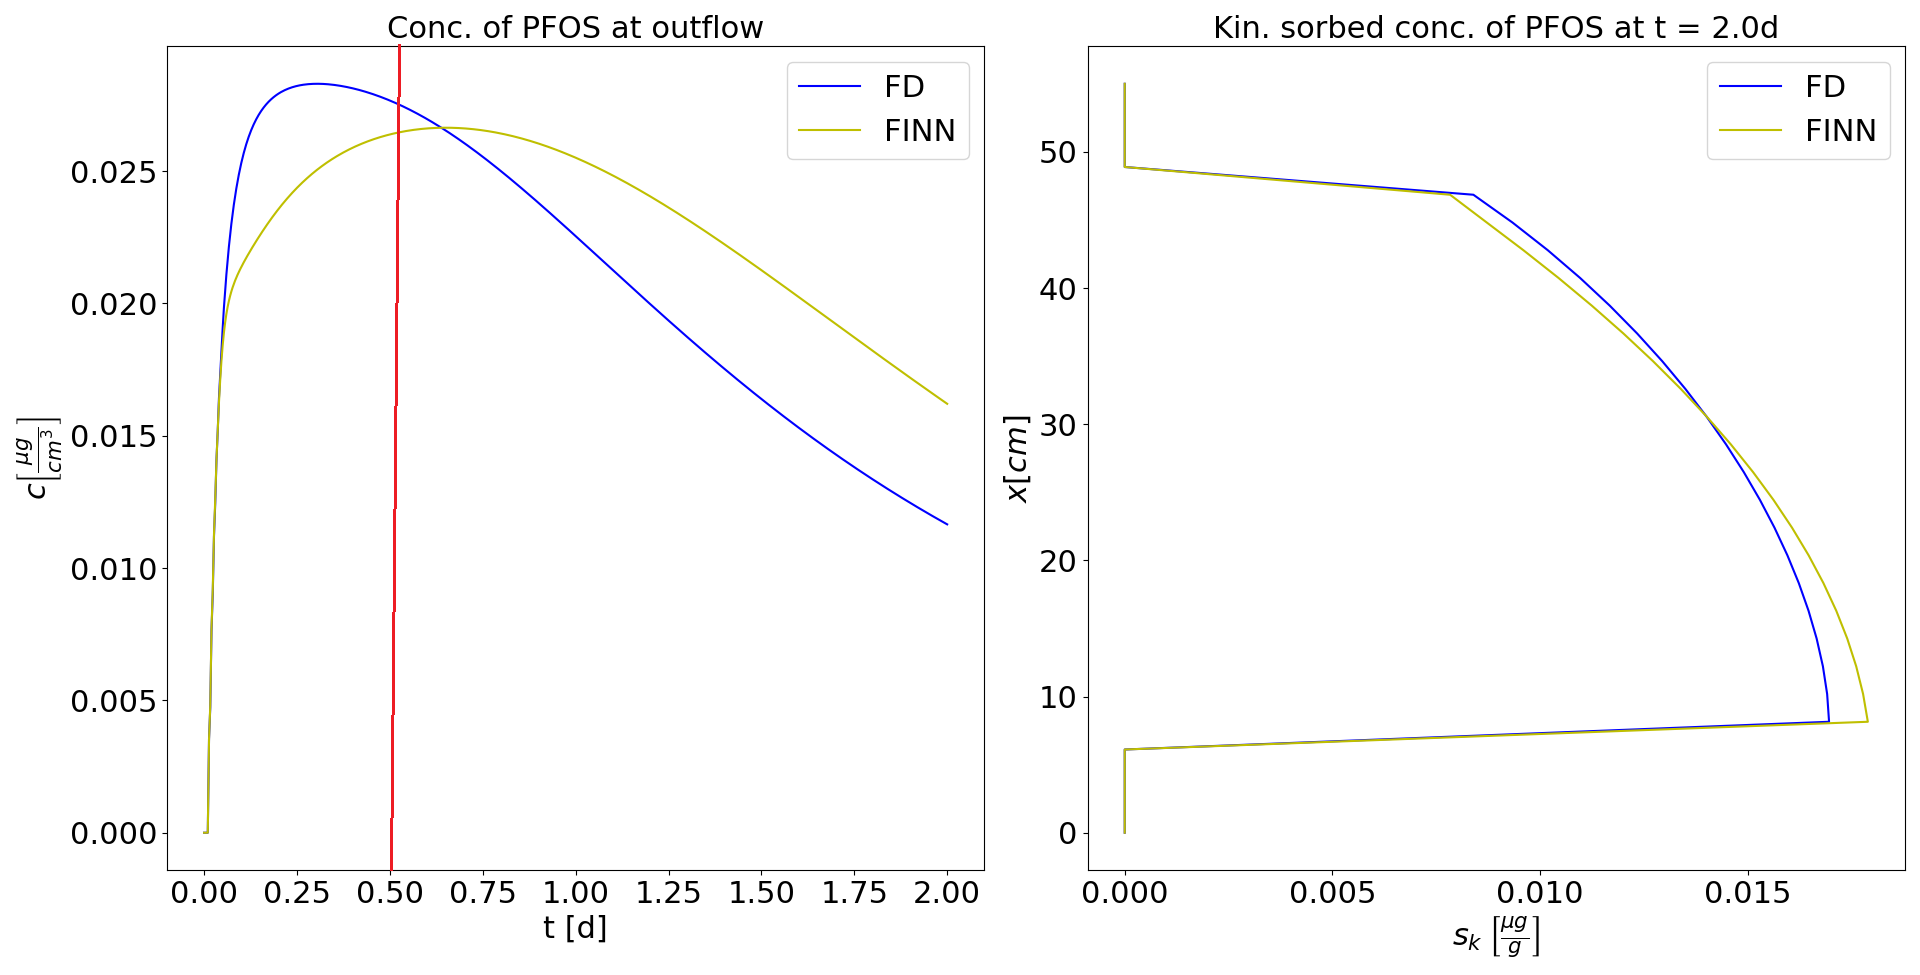
\includegraphics[scale=0.3]{images/res_btc_synt_FGR_300_m.png}
\caption[Additional comparison of FINN and FD BTCs]{BTC of PFOS given by FD and approximated by FINN (left), Kin. sorbed concentration of PFOS at $t_{end}$ (right). Red line marks the end of the training data set, 300 training epochs. Other settings as in run e.}
\label{fig:res_btc_synt_FGR_300_m}
\end{figure}
\begin{figure}
	\centering
	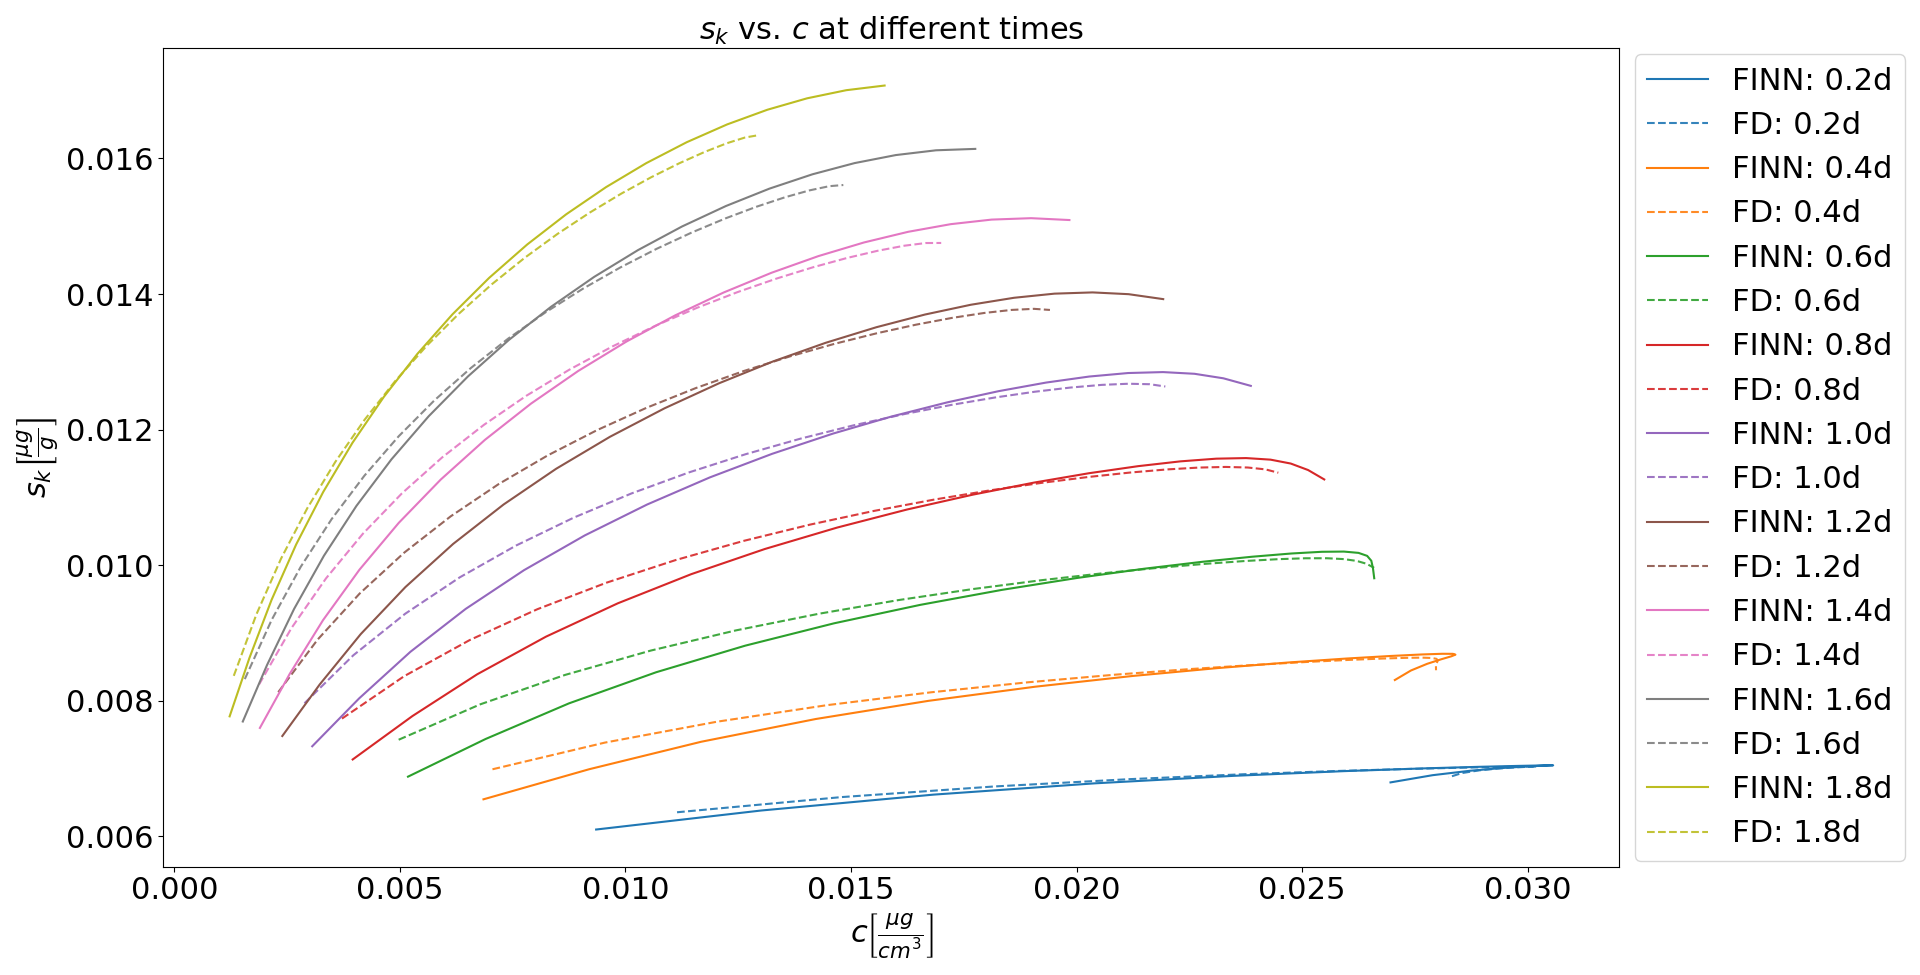
\includegraphics[scale=0.3]{images/res_sorp_synt_FGR_300.png}
\caption[Additional comparison of FINN and FD sorption behavior]{The unknowns $s_k$ and $c$ of the solution at fixed time steps, 300 training epochs. Other settings as in run e.}
\label{fig:res_sorp_synt_FGR_300}
\end{figure}